\makeatletter%
\special{pdf: put @thispage <</Group << /S /Transparency /I true /CS /DeviceRGB>> >>}%
\makeatother%
\documentclass[a4paper,twoside,10pt]{article}
\usepackage[left=2.45cm,top=2.52cm,right=1.85cm,bottom=2.95cm]{geometry}

\usepackage[xetex]{hyperref}

\usepackage{csquotes}

\usepackage[printonlyused]{acronym}

\usepackage{graphicx}
\usepackage{caption}
\usepackage{subcaption}

\usepackage{booktabs}
\usepackage{multirow}

\usepackage{amsmath}
\usepackage{txfonts}

\usepackage{minted}

\usepackage[backend=biber,style=alphabetic,natbib=true]{biblatex}
\addbibresource{bibliography.bib}

\title{Notes to Andrew Ng's Machine Learning Course}
\author{Jan Wedekind}

\begin{document}
\maketitle

\section{Introduction}

\subsection{What is Machine Learning}
These are course notes\footnote{source code here: \url{https://igit.comm.ad.roke.co.uk/jw4/machine-learning-tutorial}} to Andrew Ng's video lecture\citep{andrewng}.
A well-posed learning problem (as defined by Tom Mitchell) is:
\begin{displayquote}
  A computer program is said to \emph{learn} from experience E with respect to some task T and some performance measure P, if its performance on T, as measured by P, improves with experience E.
\end{displayquote}

Relevant software: Tensorflow\footnote{most popular machine learning software available at \url{https://www.tensorflow.org/}},
Theano\footnote{machine Learning Software available at \url{http://deeplearning.net/software/theano/}},
and Maxima\footnote{computer algebra system available at \url{http://maxima.sourceforge.net/}}.

\subsection{Supervised Learning}
\begin{figure}[htbp]
  \begin{center}
    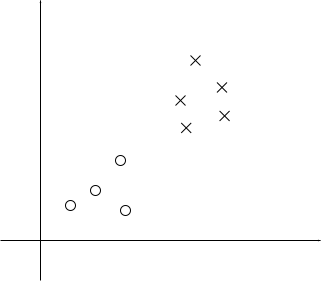
\includegraphics[width=.4\textwidth]{supervised}
    \caption{Labelled data for supervised learning\label{fig:supervised}}
  \end{center}
\end{figure}
Here are two examples for problems of different learning problems (given \emph{labelled} data as shown in Figure \ref{fig:supervised}):
\begin{itemize}
  \item Regression problem (\emph{continuous} value): estimating house price given size in square feet
  \item Classification problem (\emph{discrete} values): determine whether a tumor is malignant or benign given size of tumor and age of person
\end{itemize}

\subsection{Unsupervised Learning}
\begin{figure}[htbp]
  \begin{center}
    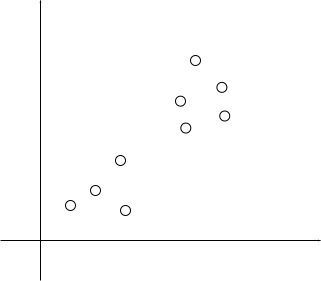
\includegraphics[width=.4\textwidth]{unsupervised}
    \caption{Data without labels\label{fig:unsupervised}}
  \end{center}
\end{figure}
When the data is not labelled (see \emph{unlabelled} data in Figure \ref{fig:unsupervised}), one can still apply clustering algorithms to it.
For example Google News clusters groups related news articles into stories.
Another basic but impressive example is separating two audio sources (speaker and a radio) using data from two microphones.

For development Andrew Ng recommends GNU Octave\citep{octave}.

\section{Linear Regression with One Variable}
\subsection{Model Representation}
\begin{table}[htbp]
  \begin{center}
    \begin{tabular}{r|r}\toprule
      \multicolumn{1}{c|}{\textbf{Size in feet$^2$ $(x)$}} &
      \multicolumn{1}{c}{\textbf{Price (\$) in 1000's $(y)$}}\\\midrule
      2104 & 460\\
      1416 & 232\\
      1534 & 315\\
       852 & 178\\
      $\vdots$ & $\vdots$\\\bottomrule
    \end{tabular}
    \caption{Table of house size and price\label{tbl:houses}}
  \end{center}
\end{table}
\newcommand{\sxi}{\ensuremath{x^{(i)}}}
\newcommand{\syi}{\ensuremath{y^{(i)}}}
\newcommand{\sumi}{\ensuremath{\displaystyle\sum_{i=1}^m}}
House price depending on house size example (see Table \ref{tbl:houses}): supervised regression problem.
The training set is denoted $(x,y)$ and the $i$th sample is $(\sxi,\syi)$ with $i\in\{1,2,\ldots,m\}$ where $m$ is the number of training samples.

The result of the learning algorithm is a \emph{hypothesis} $h$ which maps $x^\prime$ to an estimated value $y^\prime$.
\emph{E.g.} here the hypothesis is the linear function $h_\theta(x)=\theta_0+\theta_1\,x$.

Linear regression with one variable (the variable here is $x$) can also be called \emph{univariate} linear regression.

\subsection{Cost Function}\label{cha:costfunction}
The aim is to minimize the $h_\theta(x)-y$.
\emph{I.e.} minimizing the cost function (or square error function) $J(\theta_0,\theta_1)$ in the following equation
\begin{equation*}
  \displaystyle\mathop{\operatorname{argmin}}_{\theta_0,\theta_1}\underbrace{\frac{1}{2\,m}\,\sumi\big(h_\theta(\sxi)-\syi\big)^2}_{\eqqcolon J(\theta_0,\theta_1)}
\end{equation*}

\subsection{Cost Function Intuition}
With the simplified hypothesis $h_\theta(x)=\theta_1\,x$ we get
\begin{equation*}
  \theta_1=\mathop{\operatorname{argmin}}_{\theta_1}J(\theta_1)=\mathop{\operatorname{argmin}}_{\theta_1}\frac{1}{2\,m}\,\sumi\big(\theta_1\,\sxi-\syi\big)^2
\end{equation*}
The minimum can be obtained by solving for where the derivative is zero
\begin{equation*}
  \frac{\delta}{\delta\theta_1}J(\theta_1)=\frac{1}{m}\,\sumi\big(\theta_1\,\sxi-\syi\big)\,\sxi\overset{!}{=}0\Leftrightarrow
  \theta_1=\sumi\sxi\,\syi\bigg/\sumi\sxi\,\sxi
\end{equation*}
Using a contour plot one can visualise the two-dimensional version of $J(\theta_0,\theta_1)$ when using the full model.

Least-square estimation for $h_\theta(x)=\theta_0+\theta_1\,x$ yields
\begin{equation*}
\frac{1}{m}\,\sumi\big(\theta_0+\theta_1\,\sxi-\syi\big)\,\begin{pmatrix}1\\\sxi\end{pmatrix}\overset{!}{=}\vec{0}\Leftrightarrow
\begin{pmatrix}\theta_0\\\theta_1\end{pmatrix}=
\begin{pmatrix}m&\sum\sxi\\\sum\sxi&\sum\sxi\,\sxi\end{pmatrix}^{-1}\,
\begin{pmatrix}\sum\syi\\\sum\sxi\,\syi\end{pmatrix}
\end{equation*}
See Appendix \ref{app:lse} for the implementation. Figure \ref{fig:lse} shows sample data with a least square fit.
\begin{figure}[htbp]
  \begin{center}
    \includegraphics[width=.6\textwidth]{least_squares}
    \caption{Example data and corresponding least square fit of a linear function\label{fig:lse}}
  \end{center}
\end{figure}

\subsection{Gradient Descent}\label{cha:gradientdescent}
Starting from an initial solution $\theta_j$ with $j\in\{0,1\}$, the solution is updated iteratively using
\begin{equation*}
  \theta_j\coloneqq\theta_j-\alpha\,\frac{\delta}{\delta\theta_j}J(\theta_0,\theta_1)
\end{equation*}
where $\alpha$ is the learning rate.
Note that the parameters are updated ``simultaneously'' using the gradient vector $\delta J/\delta\theta$
\begin{equation}\label{equ:gradientdescent}
  \theta\coloneqq\theta-\alpha\,\frac{\delta}{\delta\theta}J(\theta)
\end{equation}

\subsection{Gradient Descent Intuition}
\begin{itemize}
  \item If $\alpha$ is too small, the algorithm will converge slowly.
  \item If $\alpha$ is too large, the algorithm will not converge on the local minimum.
\end{itemize}

\subsection{Gradient Descent for Linear Regression}
Gradient descent is performed using Equation (\ref{equ:gradientdescent}). Here the gradient is
\begin{equation*}
  \frac{\delta}{\delta\theta}J(\theta)=
  \frac{1}{m}\,\sumi\big(\theta_0+\theta_1\,\sxi-\syi\big)\,\begin{pmatrix}1\\\sxi\end{pmatrix}=
  \frac{1}{m}\,\begin{pmatrix}m&\sum\sxi\\\sum\sxi&\sum\sxi\,\sxi\end{pmatrix}\,
  \begin{pmatrix}\theta_0\\\theta_1\end{pmatrix}
\end{equation*}

See Appendix \ref{app:gradientdescent} for an implementation using symbolic differentiation of the cost function $J$.
A result of the iterative algorithm is shown in Figure \ref{fig:gradient_descent}.
\begin{figure}[htbp]
  \begin{center}
    \includegraphics[width=.6\textwidth]{gradient_descent}
    \caption{Example data and corresponding least square fit of a linear function\label{fig:gradient_descent}}
  \end{center}
\end{figure}

\section{Linear Regression with Multiple Variables}
\subsection{Multiple Features}
In the case of $n$ features, each feature $\sxi$ is a $n+1$ dimensional feature vector with $x_0$ set to $1$ for convenience:
\begin{equation*}
  \sxi=\begin{pmatrix}\sxi_0\\\sxi_1\\\vdots\\\sxi_n\end{pmatrix}\in\mathbb{R}^{n+1}
  \mathrm{\ where\ }\sxi_0\coloneqq 1
\end{equation*}
The hypothesis $h$ is
\begin{equation*}
  h_\theta(x)=\theta_0+\theta_1\,x_1+\theta_2\,x_2+\ldots+\theta_n\,x_n
\end{equation*}
Using $x_0=1$ the hypothesis can be written more compactly using the vector inner product:
\begin{equation*}
  h_\theta(x)=\theta^\top x
\end{equation*}
Regression using multiple variables is called \emph{multivariate regression}.

\subsection{Gradient Descent for Multiple Variables}\label{cha:linearregression}
The cost function $J$ can be written using vector notation
\begin{equation*}
  J(\theta)=\frac{1}{2\,m}\sumi\big(h_\theta(\sxi)-\syi\big)^2
\end{equation*}
As in Section \ref{cha:gradientdescent}, gradient descent is performed using the parameter $\alpha$:
\begin{equation*}
  \theta_j\coloneqq\theta_j-\alpha\cdot\underbrace{\frac{\delta}{\delta\theta_j}J(\theta)}_
  {\frac{1}{m}\sumi\big(h_\theta(\sxi)-\syi\big)\,\sxi}\mathrm{\ for\ }j\in\{0,\ldots,n\}
\end{equation*}

\subsection{Feature Scaling}
Feature scaling is about scaling $x_1,x_2,\ldots$ so that the variation of the values is similar.
Gradient descent then will converge more quickly (see Figure \ref{fig:scaling}).
\begin{figure}[htbp]
  \begin{center}
    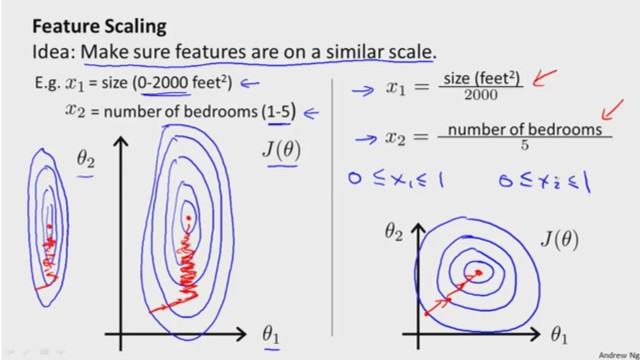
\includegraphics[width=.6\textwidth]{scaling}
    \caption{Feature scaling improves the performance of gradient descent\citep{andrewng}\label{fig:scaling}}
  \end{center}
\end{figure}
A common approach is to normalise the features to zero mean ($\mu=0$) and a standard deviation of one ($\sigma=1$).

\subsection{Learning Rate}
When performing gradient descent, $J(\theta)$ should decrease after each iteration.
Plotting $J(\theta)$ over each iteration can help to tell whether gradient descent has converged (see Figure \ref{fig:alphas}).
If $J(\theta)$ is increasing, $\alpha$ might be too large.
\begin{figure}[htbp]
  \begin{center}
    \includegraphics[width=.6\textwidth]{learning_rate}
  \caption{Plotting the cost function over the iterations can help choosing an appropriate value for the learning rate $\alpha$\label{fig:alphas}}
  \end{center}
\end{figure}

\subsection{Features and Polynomial Regression}\label{cha:polyregression}
Similar as in support vector machines one can perform linear regression on non-linear functions of features.
\emph{I.e.} given a feature $x$, one can generate additional features $x^2$, $\sqrt x$, $\ldots$.

\subsection{Normal Equation}\label{cha:normal}
An analytical solution for the linear regression problem exists since the cost function is a quadratic function and
can be written as follows
\begin{equation*}
  J(\theta)=a\,\theta^2+b\,\theta+c
\end{equation*}
An analytical solution for minimizing $J$ can be found by solving the following equation system
\begin{equation*}
  \frac{\delta}{\delta\theta_j}J(\theta)=0
\end{equation*}
The least squares problem is written in the following form.
\begin{equation*}
  \underbrace{\begin{pmatrix}
1&x^{(1)}_1&x^{(1)}_2&\hdots&x^{(1)}_n\\
1&x^{(2)}_1&x^{(2)}_2&\hdots&x^{(2)}_n\\
\vdots&\vdots&\vdots&\ddots&\vdots\\
1&x^{(m)}_1&x^{(m)}_2&\hdots&x^{(m)}_n
  \end{pmatrix}}_{\coloneqq\mathcal{X}}\,\theta=
\underbrace{\begin{pmatrix}y^{(1)}\\\vdots\\y^{(m)}\end{pmatrix}}_{y}+\epsilon
\end{equation*}
The solution is $\theta=(\mathcal{X}^\top\mathcal{X})^{-1}\mathcal{X}^\top y$.

\subsection{Normal Equation Non Invertibility}
There are two cases where the least square solution $\theta=(\mathcal{X}^\top\mathcal{X})^{-1}\mathcal{X}^\top y$ is not invertible
\begin{itemize}
  \item redundant (linear dependent) features
  \item too many features (\emph{e.g.} more features than data, $m\le n$)
    \begin{itemize}
      \item delete some features or
      \item use regularisation
    \end{itemize}
\end{itemize}
The closed solution is preferable if the number of features $n$ is small (see Figure \ref{fig:gcp}).
\begin{figure}[htbp]
  \begin{center}
    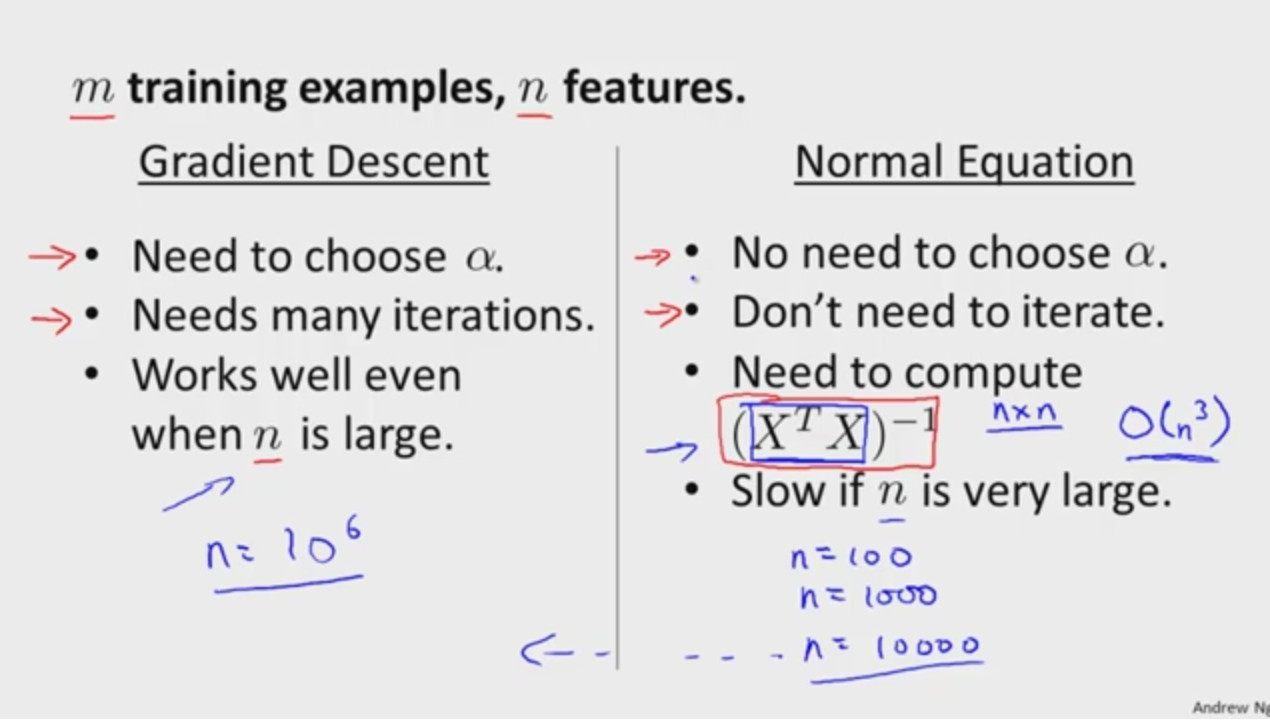
\includegraphics[width=.6\textwidth]{gradientproscons}
    \caption{Pros and cons for using gradient descent instead of the normal equation\citep{andrewng}\label{fig:gcp}}
  \end{center}
\end{figure}

\section{Logistic Regression}
\subsection{Classification}
The basic case is the binary classification problem $y\in\{0,1\}$.
Applying linear regression and thresholding the result (\emph{e.g.} $h_\theta(x)\ge 0.5$ generally does not perform well.
$0\le h_\theta(x)\le 1$ is not fullfilled for most linear models.

\subsection{Hypothesis Representation}
The logistic regression model uses the \emph{sigmoid} function (or \emph{logistic} function).
\begin{equation*}
  h_\theta(x)=g(\theta^\top x)\mathrm{\ where\ }g(z)=\frac{1}{1+\operatorname{e}^{-z}}
\end{equation*}
\begin{figure}[htbp]
  \begin{center}
    \includegraphics[width=.4\textwidth]{sigmoid}
    \caption{Sigmoid function\label{fig:sigmoid}}
  \end{center}
\end{figure}
Figure \ref{fig:sigmoid} shows the characteristic ``S''-shaped curve of the sigmoid function\footnote{\url{https://en.wikipedia.org/wiki/Sigmoid_function}}.
The model based on the sigmoid function is
\begin{equation*}
  h_\theta(x)=\frac{1}{1+\operatorname{e}^{-\theta^\top x}}
\end{equation*}
The output of $h_\theta(x)$ is interpreted as the estimated probability that $y=1$ on input $x$.
\begin{equation*}
  h_\theta(x)=P(y=1|\,x;\theta)
\end{equation*}

\subsection{Decision Boundary}
The prediction is
\begin{itemize}
  \item ``$y=1$'' if $h_\theta(x)\ge 0.5$
  \item ``$y=0$'' if $h_\theta(x)<0.5$
\end{itemize}
With $h_\theta(x)=g(\theta^\top x)$ and $g$ being monotonous, this is equivalent to
\begin{itemize}
  \item ``$y=1$'' if $\theta^\top x\ge 0$
  \item ``$y=0$'' if $\theta^\top x< 0$
\end{itemize}
The decision boundary in this case is a hyperplane in the feature space. \emph{E.g.} given two features
\begin{equation*}
  h_\theta(x)=g(\theta_0+\theta_1\,x_1+\theta_2\,x_2)
\end{equation*}
the decision boundary is
\begin{equation*}
  \theta_0+\theta_1\,x_1+\theta_2\,x_2=0
\end{equation*}
\begin{figure}[htbp]
  \begin{center}
    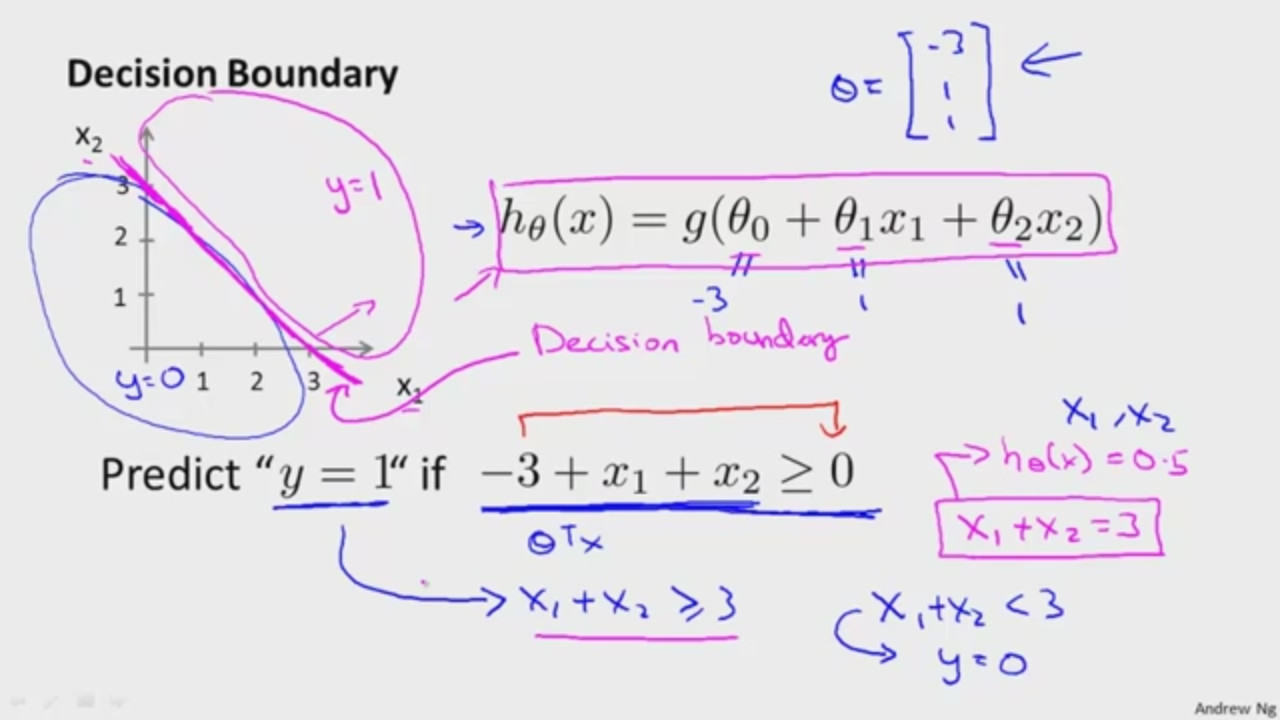
\includegraphics[width=.6\textwidth]{decisionboundary}
    \caption[Linear decision boundary]{Linear decision boundary. ``x'' denotes a positive sample (y=1) and ''o'' a negative sample (y=1)\citep{andrewng}\label{fig:decisionboundary}}
  \end{center}
\end{figure}
It separates the ``y=1'' region and the ``y=0'' region (also see Figure \ref{fig:decisionboundary}).

\begin{figure}[htbp]
  \begin{center}
    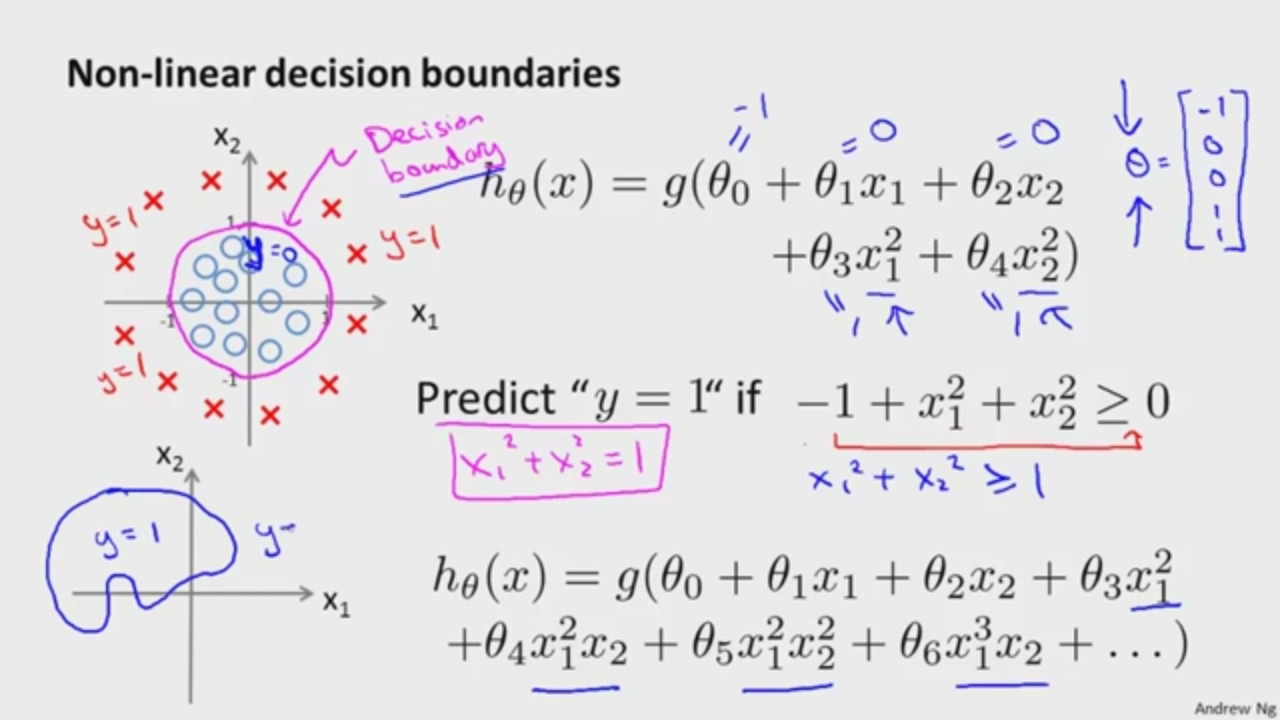
\includegraphics[width=.6\textwidth]{circularboundary}
    \caption{Circular decision boundary\citep{andrewng}\label{fig:circularboundary}}
  \end{center}
\end{figure}
Similar as in Section \ref{cha:polyregression} one can use polynomial terms to introduce additional features in order to achieve a non-linear decision boundary (see Figure \ref{fig:circularboundary}). \emph{E.g.} one can use a circular decision boundary in the hypothesis
\begin{equation*}
  h_\theta(x)=g(\underbrace{\theta_0}_{=-1}+\underbrace{\theta_1}_{=0}\,x_1+\underbrace{\theta_2}_{=0}\,x_2+\underbrace{\theta_3}_{=1}\,x_1^2+\underbrace{\theta_4}_{=1}\,x_2^2)
\end{equation*}

\subsection{Cost Function}
Given
\begin{itemize}
\item a training set of $m$ training examples $\{(x^{(1)},y^{(1)},x^{(2)},y^{(2)},\ldots,x^{(m)},y^{(m)}\}$ with
$x\in\begin{pmatrix}x_0\\x_1\\\vdots\\x_n\end{pmatrix}$, $x_0=1$, $y\in\{0,1\}$
\item a hypothesis $h_\theta(x)=\displaystyle\frac{1}{1+\operatorname{e}^{-\theta^\top x}}$
\end{itemize}
Desired is a parameter vector $\theta$ so that $h_\theta(x)$ produces good predictions.

The cost function introduced in Section \ref{cha:costfunction} is generalised as follows
\begin{equation*}
  J(\theta)=\frac{1}{m}\sumi Cost(h_\theta(\sxi),\syi)
\end{equation*}
In the case of linear regression the cost function is $cost(h_\theta(x),y)=\frac{1}{2}(h_\theta(x)-y)^2$.
In the case of logistic regression this function would be ``non-convex''. Instead the following cost function is used
\begin{equation*}
Cost(h_\theta(x),y)=
\left\{\begin{array}{rl}-\operatorname{log}(h_\theta(x))&\mathrm{if\ }y=1\\
-\operatorname{log}(1-h_\theta(x))&\mathrm{if\ }y=0\end{array}\right.
\end{equation*}
\begin{figure}[htbp]
  \begin{center}
    \begin{subfigure}[b]{.47\textwidth}
      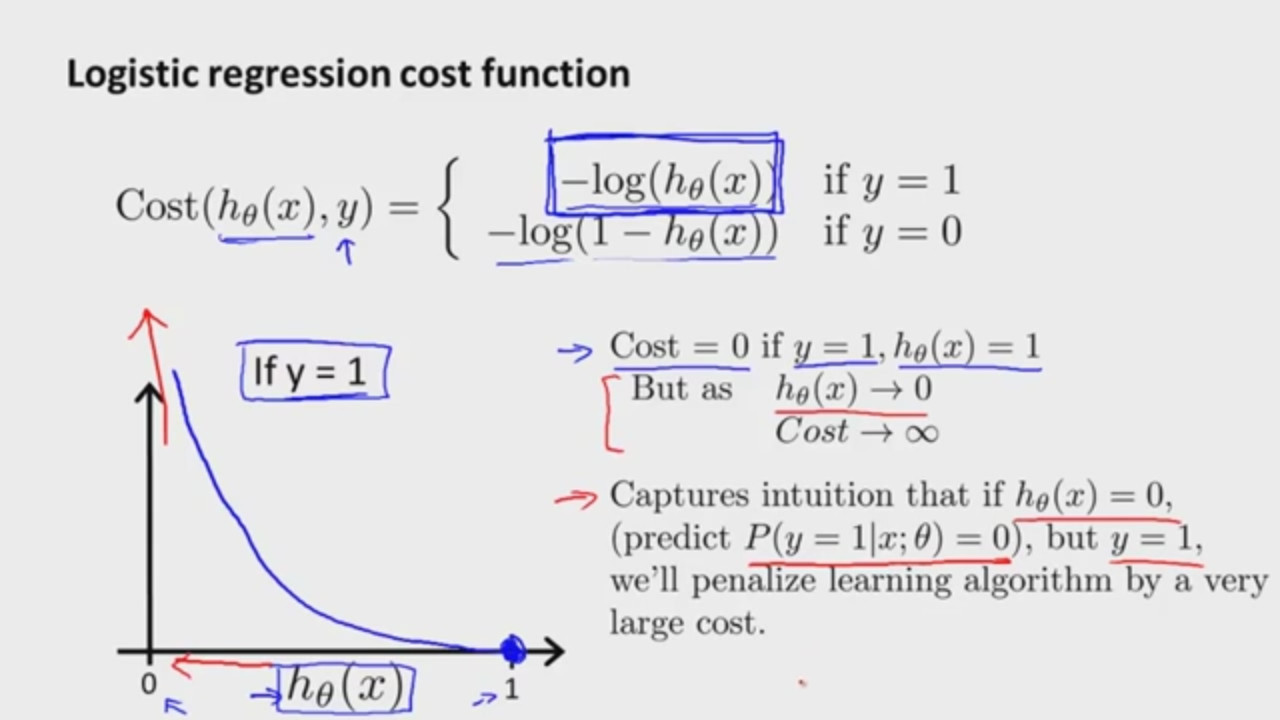
\includegraphics[width=\linewidth]{costy1}
      \caption{Cost function for ``y=1''}
    \end{subfigure}
    \begin{subfigure}[b]{.47\textwidth}
      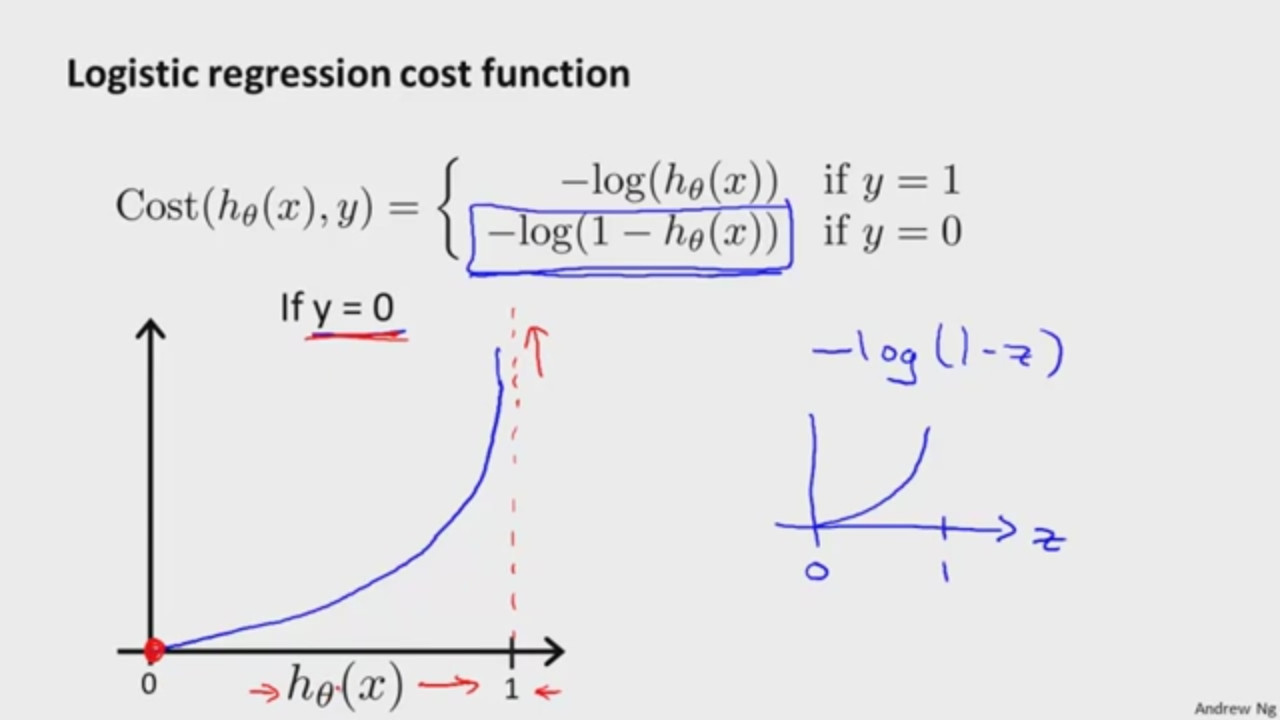
\includegraphics[width=\linewidth]{costy0}
      \caption{Cost function for ``y=0''}
    \end{subfigure}
    \caption{Cost function for logistic regression\citep{andrewng}\label{fig:costlog}}
  \end{center}
\end{figure}
See Figure \ref{fig:costlog} for a visualisation.

\subsection{Simplified Cost Function and Gradient Descent}
The cost function
\begin{equation*}
Cost\big(h_\theta(x),y\big)=
\left\{\begin{array}{rl}-\operatorname{log}\big(h_\theta(x)\big)&\mathrm{if\ }y=1\\
-\operatorname{log}\big(1-h_\theta(x)\big)&\mathrm{if\ }y=0\end{array}\right.
\end{equation*}
can be rewritten as follows
\begin{equation*}
Cost\big(h_\theta(x),y\big)=
-y\,\operatorname{log}\big(h_\theta(x)\big)-(1-y)\,\operatorname{log}\big(1-h_\theta(x)\big)
\end{equation*}
The overall cost function $J(\theta)$ is\footnote{similar as in maximum likelihood estimation}
\begin{equation*}
  J(\theta)=-\frac{1}{m}\big[\sumi\syi\operatorname{log}h_\theta(\sxi)+(1-\syi)\operatorname{log}(1-h_\theta(\sxi))\big]
\end{equation*}

The minimization problem $\mathop{\operatorname{argmin}}_\theta J(\theta)$ can be solved using gradient descent
\begin{equation*}
  \theta_j\coloneqq\theta_j-\alpha\cdot\underbrace{\frac{\delta}{\delta\theta_j}J(\theta)}_
  {=\frac{1}{m}\sumi\big(h_\theta(\sxi)-\syi\big)\,\sxi}
\end{equation*}
Note that the choice of $h_\theta(x)=\frac{1}{1+\operatorname{e}^{-\theta^\top x}}$ for logistic regression has led to the \emph{same} gradient descent rule as used for linear regression (with $h_\theta(x)=\theta^\top x$ as shown in Section \ref{cha:linearregression}).

See Figure \ref{fig:classifier} for an example of classifying binary data with two features.
The corresponding implementation is shown in Appendix \ref{app:classifier}.
\begin{figure}[htbp]
  \begin{center}
    \includegraphics[width=.6\textwidth]{classifier}
    \caption{Classifying binary data with two features\label{fig:classifier}}
  \end{center}
\end{figure}

Figure \ref{fig:polynomial} shows an example using polynomial (non-linear) features (see Appendix \ref{app:polynomial} for implementation).
\begin{figure}[htbp]
  \begin{center}
    \includegraphics[width=.6\textwidth]{polynomial}
    \caption{Classifying binary data using polynomial features\label{fig:polynomial}}
  \end{center}
\end{figure}

\subsection{Advanced Optimization}
There are other algorithms for optimizing the cost functions given
\begin{itemize}
  \item the cost function $J(\theta)$
  \item the derivative $\frac{\delta}{\delta\theta_j}J(\theta)$
\end{itemize}
Some optimization algorithms are
\begin{itemize}
  \item Gradient descent
  \item Conjugate gradient
  \item \acs{BFGS}\footnote{\url{https://en.wikipedia.org/wiki/Broyden\%E2\%80\%93Fletcher\%E2\%80\%93Goldfarb\%E2\%80\%93Shanno_algorithm}}
  \item \acs{L-BFGS}\footnote{\url{https://en.wikipedia.org/wiki/Limited-memory_BFGS}}
\end{itemize}
More advanced algorithms have the following advantages
\begin{itemize}
  \item no need to manually pick $\alpha$
  \item often converge faster than gradient descent
\end{itemize}
However the algorithms are more complex. It is not recommended to implement this algorithms yourself.

\subsection{Multi-Class Classification: One-vs-all}\label{cha:onevsall}
The binary classifier can be generalised to multi-class problems using multiple one-vs-all classifiers.
\emph{E.g.} for $y\in\{1,2,3\}$ three classifiers $h_\theta^{(i)}(x)=P(y=i\|\,x;\theta)$ for $i\in\{1,2,3\}$ are trained.
To make a prediction, the classifier outputting the highest probability is selected (see Figure \ref{fig:onevsall}):
\begin{equation*}
  \mathop{\operatorname{max}}_ih_\theta^{(i)}(x)
\end{equation*}
\begin{figure}[htbp]
  \begin{center}
    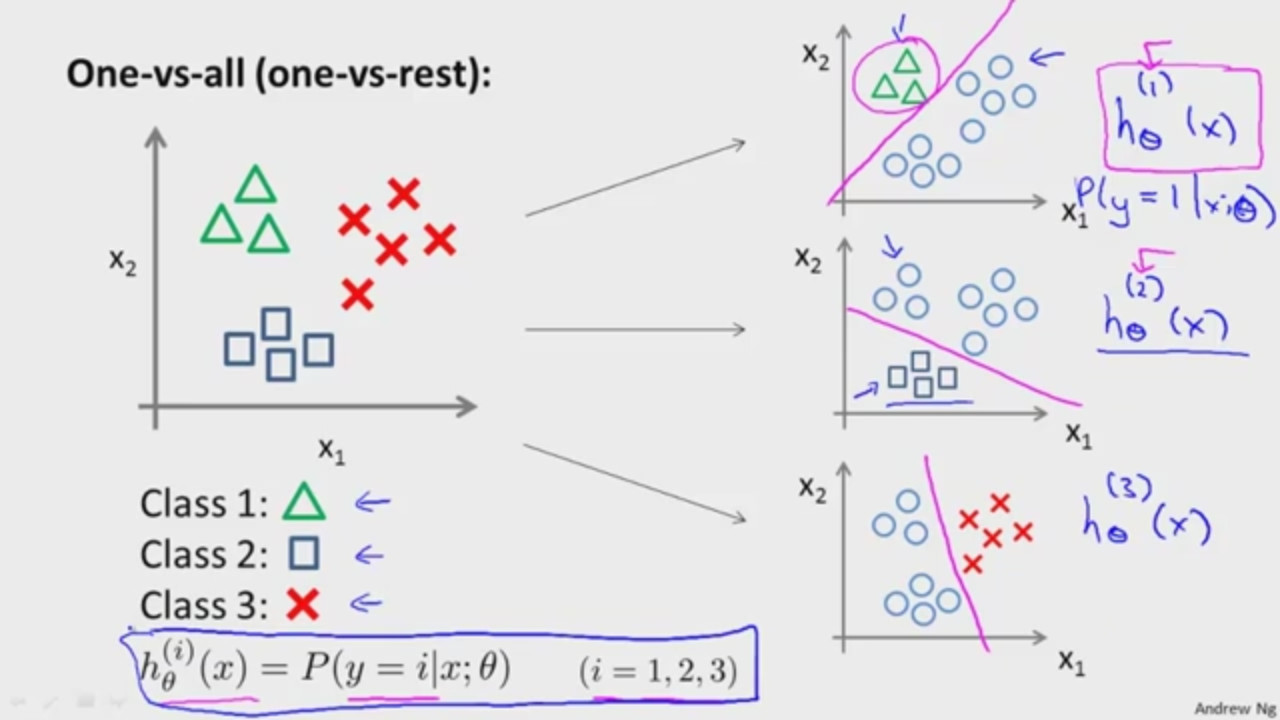
\includegraphics[width=.6\textwidth]{onevsall}
    \caption{Multi-class classification using one-vs-all classifiers\citep{andrewng}\label{fig:onevsall}}
  \end{center}
\end{figure}

\section{Regularization}
\subsection{The Problem of Overfitting}
\begin{itemize}
  \item If the model is \textbf{underfit}, there is a poor fit to the data causing a \emph{high bias}.
  \item The other extreme is an \textbf{overfit} model with too many parameters causing high \emph{high variance}.
\end{itemize}
If the data is overfit, the fit is very well (low value for $J(\theta)$) but it fails to generalize to new examples.
See Figure \ref{fig:overfitting} for an eample of overfitting (implementation in Appendix \ref{app:overfitting}).
\begin{figure}[htbp]
  \begin{center}
    \includegraphics[width=.6\textwidth]{overfitting}
    \caption{Example of overfitting\label{fig:overfitting}}
  \end{center}
\end{figure}

One can address overfitting by
\begin{enumerate}
  \item reduce number of features
    \begin{itemize}
      \item manually select features to keep
      \item model selection algorithm
    \end{itemize}
  \item regularization
    \begin{itemize}
      \item keep all the features, but reduce magnitude/values of parameters $\theta_j$
      \item works well when we have a lot of features, each of which contributes a bit to predicting $y$
    \end{itemize}
\end{enumerate}

\subsection{Cost Function}
The cost function can be modified to penalize large values for parameters.
The cost function is modified as follows
\begin{equation*}
  J(\theta)=\frac{1}{2\,m}\,\bigg[\sumi\big(h_\theta(\sxi)-\syi\big)^2+\underbrace{\lambda\,\sum_{i=1}^n\theta_j^2\bigg]}_{\mathrm{regularization\ term}}
\end{equation*}
where $\lambda$ is the \emph{regularization parameter}.
Note that by convention $\theta_0$ (constant component of the model) is not regularized.
The regularization parameters controls the trade-off between a good model fit and a regular model.

For $\lambda=0$ the cost function is the same as before which is prone to overfitting. For $\lambda\rightarrow\infty$ the resulting hypothesis converges to the constant model $h_\theta(x)=\theta_0$ and underfitting occurs.

\subsection{Regularized Linear Regression}
Applying the gradient descent algorithm to the regularized cost function results in the following update rule
\begin{align*}
  \begin{split}
    \theta_0\coloneqq&\theta_0-\alpha\,\frac{1}{m}\sumi\big(h_\theta(\sxi)-\syi\big)\,\sxi_0\\
    \theta_j\coloneqq&\theta_j-\alpha\,\frac{1}{m}\sumi\big(h_\theta(\sxi)-\syi\big)\,\sxi_j-\alpha\,\frac{\lambda}{m}\theta_j=\\
    &\theta_j\,(1-\alpha\,\frac{\lambda}{m})-\alpha\,\frac{1}{m}\sumi\big(h_\theta(\sxi)-\syi\big)\,\sxi_j
    \mathrm{\ for\ }j\in\{1,2,3,\ldots,n\}
  \end{split}
\end{align*}
The term $(1-\alpha\frac{\lambda}{m})$ equals $1-\epsilon$ with $\epsilon>0$ being a small value which shrinks each parameter towards zero at each step.

The normal equation introduced in Section \ref{cha:normal} becomes
\begin{equation*}
  \theta=\Bigg(\mathcal{X}^\top\mathcal{X}+\lambda\,
\begin{pmatrix}
  0&0&\hdots&0\\
  0&1&\ddots&\vdots\\
  \vdots&\ddots&\ddots&0\\
  0&\hdots&0&1
\end{pmatrix}\Bigg)^{-1}\mathcal{X}^\top y
\end{equation*}
In the case of $m\le n$ (fewer examples than features), $\mathcal{X}^\top\mathcal{X}$ is still invertible.

\subsection{Regularized Logistic Regression}\label{cha:regreg}
In the case of logistic regression the cost function is modified to
\begin{equation*}
  J(\theta)=-\frac{1}{m}\bigg[\sumi\syi\operatorname{log}h_\theta(\sxi)+(1-\syi)\operatorname{log}\big(1-h_\theta(\sxi)\big)\bigg]+
  \frac{\lambda}{2\,m}\sum_{j=1}^n\theta_j^2
\end{equation*}
Note that the bias unit $\theta_0$ is not regularized.

The gradient descent algorithm becomes
\begin{align*}
  \begin{split}
    \theta_0\coloneqq&\theta_0-\alpha\,\frac{1}{m}\sumi\big(h_\theta(\sxi)-\syi\big)\,\sxi_0\\
    \theta_j\coloneqq&\theta_j-\alpha\,\underbrace{\bigg[\frac{1}{m}\sumi\big(h_\theta(\sxi)-\syi\big)\,\sxi_j+\frac{\lambda}{m}\theta_j\bigg]}_{=\frac{\delta}{\delta\theta_j}J(\theta)}
    \mathrm{\ for\ }j\in\{1,2,3,\ldots,n\}
  \end{split}
\end{align*}
Note that the hypothesis here is $h_\theta(x)=\frac{1}{1+\operatorname{e}^{-\theta^\top x}}$.

\section{Neural Networks Representation}
\subsection{Non Linear Hypotheses}
Using polynomial features as shown in Section \ref{cha:polyregression} does not scale well with the number of features.
When applying logistic regression to image processing, each camera pixel is a feature.
\emph{E.g.} a $50\times 50$ image results in 2500 features (or 7500 features when using RGB images).

\subsection{Neurons and the Brain}
Using rewiring and other experiments neurologists have shown that any part of a brain can learn different tasks.
The motivation behind neural networks is to find a generic algorithm which can be applied to a variety of problems.

\subsection{Model Representation}
The neuron is modelled as a logistic unit as shown in Figure \ref{fig:logisticunit}.
\begin{figure}[htbp]
  \begin{center}
    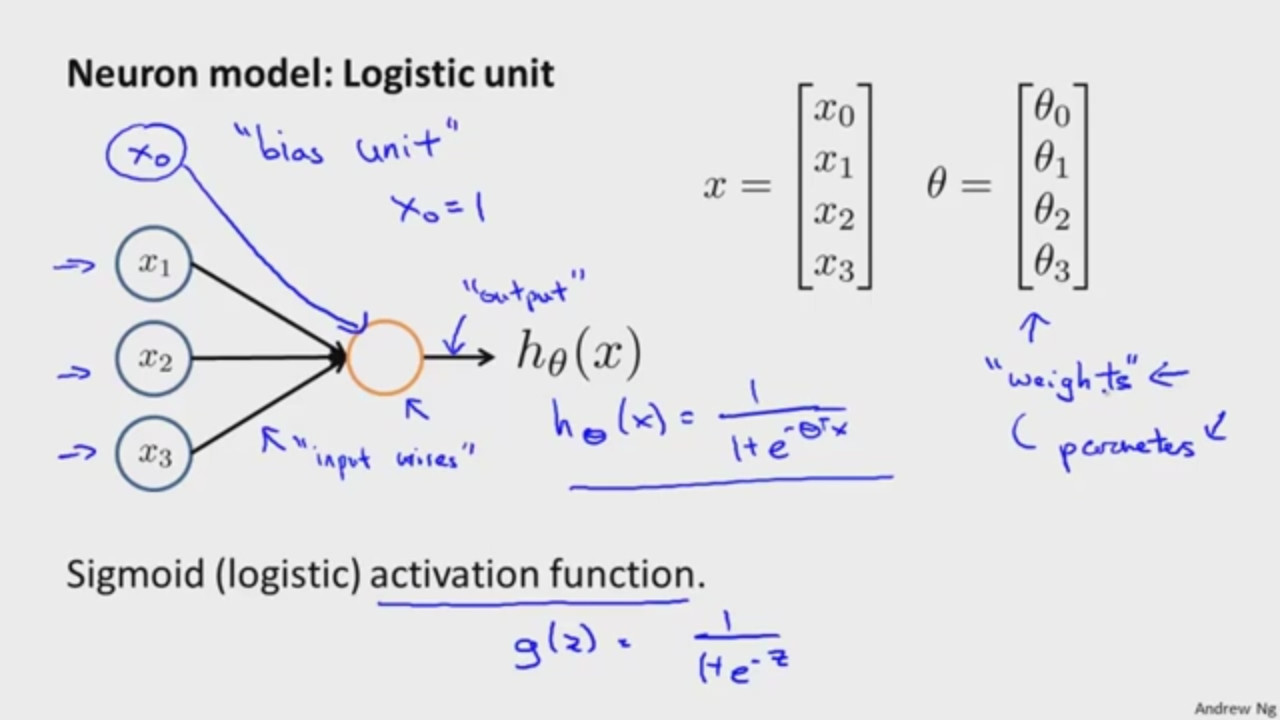
\includegraphics[width=.6\textwidth]{logisticunit}
    \caption{Modelling a neuron as a logistic unit\citep{andrewng}\label{fig:logisticunit}}
  \end{center}
\end{figure}
$x_1, x_2, \ldots$ are called ``input units'' and $x_0$ is the ``bias unit''.
$h_\theta(x)$ is the ``output''.
The sigmoid function $g(z)=\frac{1}{1+\operatorname{e}^{-z}}$ is named ``activation function''.
The components of the parameter vector $\theta$ can be called ``weights''.

A \emph{neural network} computes the output from a hidden layer instead (see Figure \ref{fig:hidden}) and can learn its own features.
\begin{figure}[htbp]
  \begin{center}
    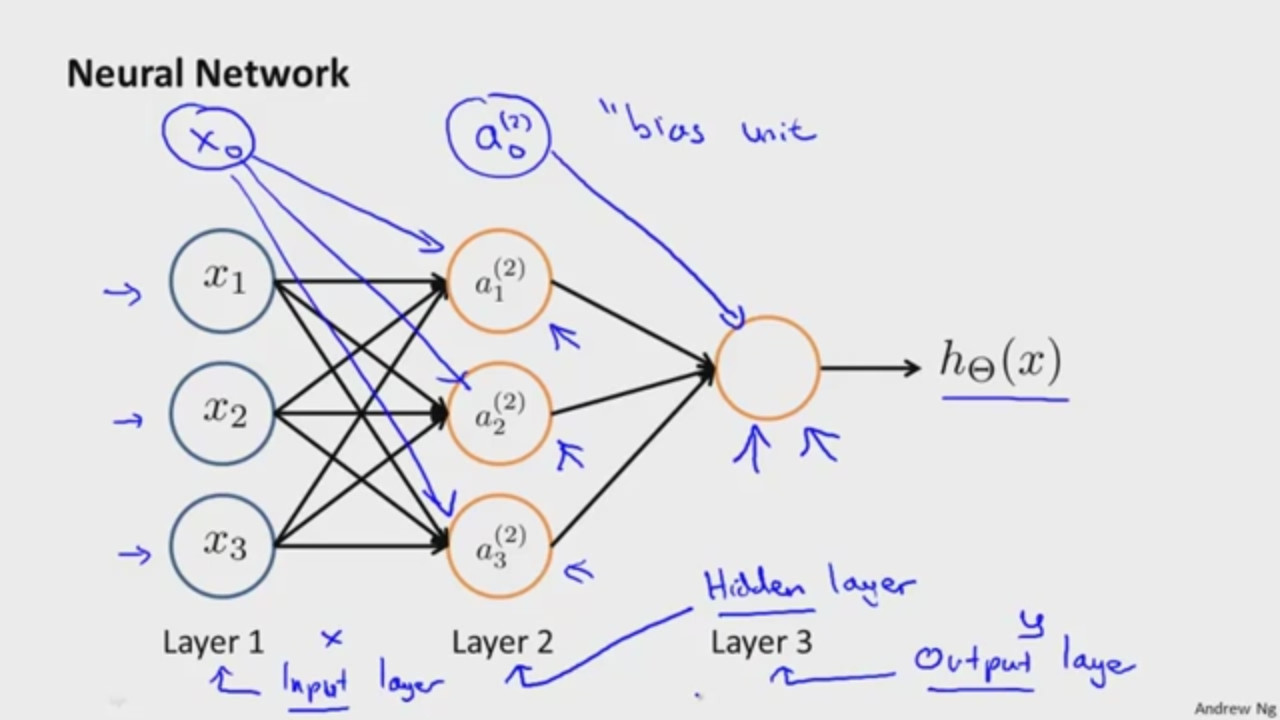
\includegraphics[width=.6\textwidth]{hidden}
    \caption{Neural network with a hidden layer\citep{andrewng}\label{fig:hidden}}
  \end{center}
\end{figure}
Additional definitions are introduced
\begin{itemize}
  \item $a^{(j)}_i\in[0,1]$ ``activation'' of unit $i$ in layer $j\ge 2$ (with bias unit $a^{(j)}_0=1$)
  \item $\theta^{(j)}\in\mathbb{R}^{s_{j+1}\times(s_j+1)}$ matrix of weights controlling function mapping from layer $j$ to layer $j+1$
  \item $s_j$ is the number of units in layer $j$
\end{itemize}
When there is one hidden layer, \emph{forward propagation} is performed as follows.
The activations of units in layer $j+1$ are determined using matrix multiplication with $\theta^{(j)}$
\begin{align*}
  \begin{split}
    a^{(2)}_0&=1\\
    a^{(2)}_1&=g(\underbrace{\theta^{(1)}_{10}\,x_1+\theta^{(1)}_{11}\,x_1+\ldots}_{=z^{(2)}_1})\\
    a^{(2)}_2&=g(\underbrace{\theta^{(1)}_{20}\,x_1+\theta^{(1)}_{21}\,x_1+\ldots}_{=z^{(2)}_2})\\
    &\vdots
  \end{split}
\end{align*}
The output is determined from the last hidden layer
\begin{equation*}
  h_\theta(x)=g(\theta^{(2)}_{10}\,a^{(2)}_0+\theta^{(2)}_{11}\,a^{(2)}_1+\theta^{(2)}_{12}\,a^{(2)}_2+\ldots)
\end{equation*}
The definition is made more compact using vectorized expressions
\begin{itemize}
  \item $z^{(2)}=\theta^{(1)}\,x\in\mathbb{R}^{s_2}$
  \item $a^{(2)}=g(z^{(2)})$ with $a^{(2)}_0=1$ ($a^{(2)}\in\mathbb{R}^{s_2+1}$)
\end{itemize}
where the definition of the digmoid function $g$ is extended to work element-wise on vectors and prepend $1$ as the first element.
The output is determined as follows
\begin{equation*}
  h_\theta(x)=a^{(3)}=g(z^{(3)})
\end{equation*}

Essentially a neural network uses more than one logistical regression layer.
Neural networks can have more than three layers. \emph{E.g.} a network with four layers
\begin{itemize}
  \item [Layer 1:] Input
  \item [Layer 2:] Hidden layer
  \item [Layer 3:] Hidden layer
  \item [Layer 4:] Output
\end{itemize}

\subsection{Examples and Intuitions}
Given two inputs (and the bias unit) one can approximate a logical ``and'' operation as follows
\begin{equation*}
  h_\theta(x)=g(-30+20\,x_1+20\,x_2)
\end{equation*}
The result is shown in the following table
\begin{center}
  \begin{tabular}{cc|c}
    $x_1$ & $x_2$ & $h_\theta(x)$\\\hline
    0 & 0 & 0.000\\
    0 & 1 & 0.000\\
    1 & 0 & 0.000\\
    1 & 1 & 1.000\\
  \end{tabular}
\end{center}
In the same fashion one can approximate a logical ``or''
\begin{equation*}
  h_\theta(x)=g(-10+20\,x_1+20\,x_2)
\end{equation*}
The result is shown in the table below
\begin{center}
  \begin{tabular}{cc|c}
    $x_1$ & $x_2$ & $h_\theta(x)$\\\hline
    0 & 0 & 0.000\\
    0 & 1 & 1.000\\
    1 & 0 & 1.000\\
    1 & 1 & 1.000\\
  \end{tabular}
\end{center}
Logical ``not'' can be approximated as follows
\begin{equation*}
  h_\theta(x)=g(10-20\,x_1)
\end{equation*}
Resulting in the desired behaviour as shown in the table below
\begin{center}
  \begin{tabular}{cc|c}
    $x_1$ & $h_\theta(x)$\\\hline
    0 & 1.000\\
    1 & 0.000\\
  \end{tabular}
\end{center}
``(not $x_1$) and (not $x_2$)'' can be implemented using
\begin{equation*}
  h_\theta(x)=g(10-20\,x_1-20\,x_2)
\end{equation*}

``($x_1$ xnor $x_2$)'' (not exclusive-or) requires a hidden layer.
The hidden layer computes the logical ``and'' and the logical ``nor''.
The activations of the hidden layer are combined using a logical ``or''.
See table below for the different states of the neural network
\begin{center}
  \begin{tabular}{cccc|c}
    $x_1$ & $x_2$ & $a^{(2)}_1$ & $a^{(2)}_2$ & $h_\theta(x)$\\\hline
    0 & 0 & 0 & 1 & 1.000\\
    0 & 1 & 0 & 0 & 0.000\\
    1 & 0 & 0 & 0 & 0.000\\
    1 & 1 & 1 & 0 & 1.000\\
  \end{tabular}
\end{center}
\emph{I.e.} to implement ``xnor'' we use
\begin{itemize}
\item $\theta^{(1)}=\begin{pmatrix}-30&20&20\\10&-20&-20\end{pmatrix}$ and
\item $\theta^{(2)}=\begin{pmatrix}-10&20&20\end{pmatrix}$
\end{itemize}
The neural network is visualised in Figure \ref{fig:xnor}.
\begin{figure}[htbp]
  \begin{center}
    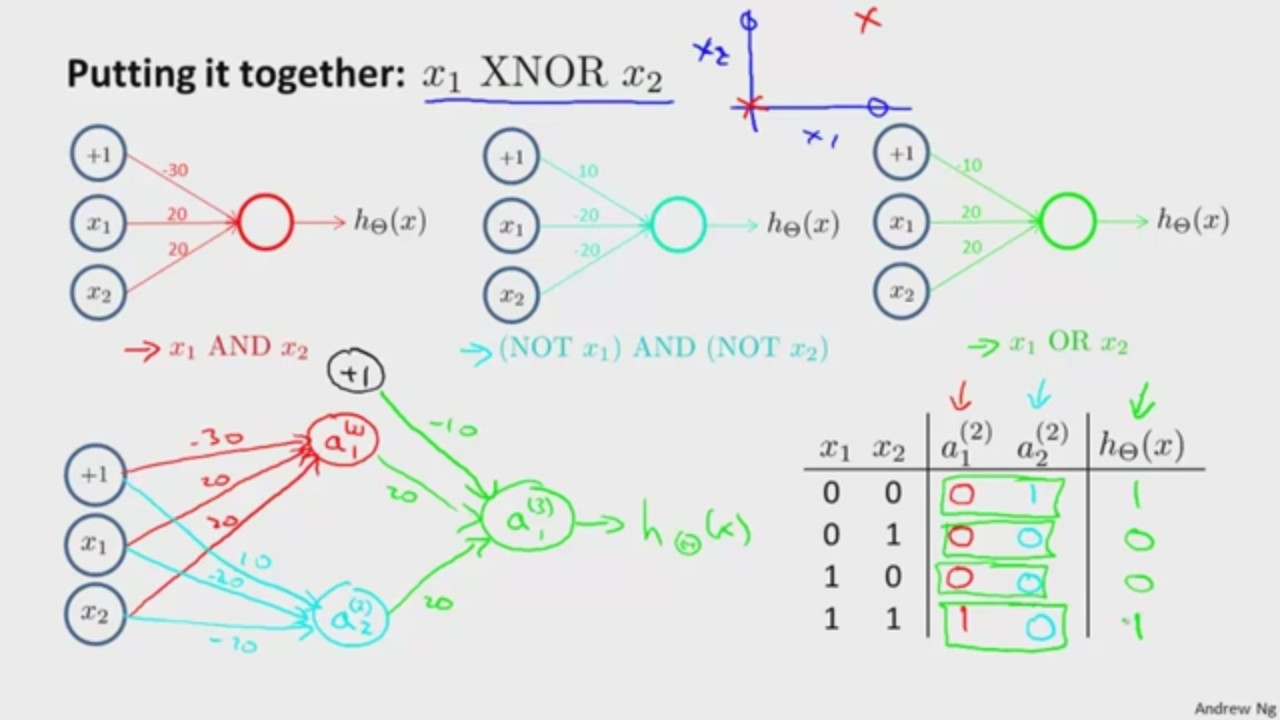
\includegraphics[width=.6\textwidth]{xnor}
    \caption{Logical ``xnor'' implemented with a neural network\citep{andrewng}\label{fig:xnor}}
  \end{center}
\end{figure}

Neural networks can be used for complex tasks such as handwritten digit classification\citep{lecun} (see Figure \ref{fig:lecun}).
\begin{figure}[htbp]
  \begin{center}
    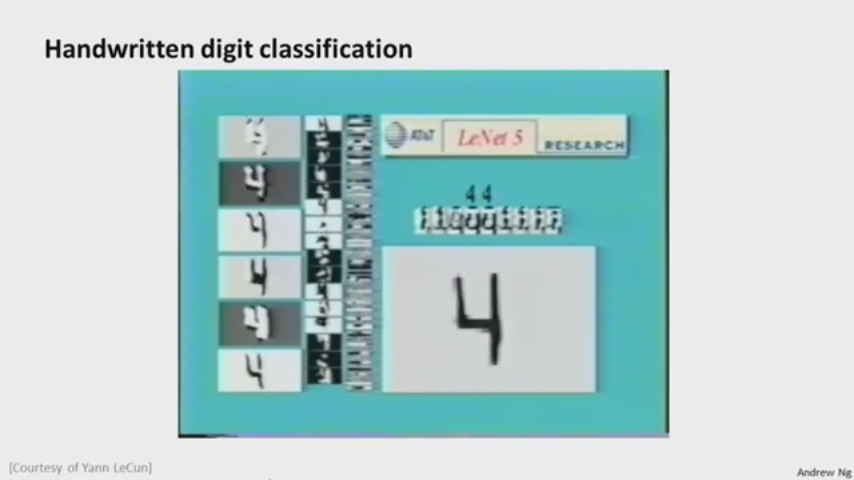
\includegraphics[width=.6\textwidth]{lecun}
    \caption{Handwritten character recognition using neural network\citep{lecun}\label{fig:lecun}}
  \end{center}
\end{figure}


\subsection{Multi-Class Classification}\label{cha:multiclassif}
Multi-class classification with neural networks is an extension of the one-vs-all method (see Section \ref{cha:onevsall}).
Basically the desired output is specified to be a unit vector.
\emph{E.g.} the desired outputs (and training labels $\syi$) for four classes ($K=4$) are
\begin{itemize}
  \item $h_\theta(x)\approx\begin{pmatrix}1\\0\\0\\0\end{pmatrix}$ for class one
  \item $h_\theta(x)\approx\begin{pmatrix}0\\1\\0\\0\end{pmatrix}$ for class two
  \item $h_\theta(x)\approx\begin{pmatrix}0\\0\\1\\0\end{pmatrix}$ for class three
  \item $\ldots$
\end{itemize}
The desired training result is $h_\theta(\sxi)\approx\syi$ with $\syi\in\mathbb{R}^K$ and $K=4$.

\subsection{Cost Function}
\begin{itemize}
  \item $L$ is the total number of layers of the network
  \item $s_l$ is the number of units in layer $l\in\{1,2,\ldots,L\}$
  \item $K=s_L$ is the number of output units
  \item $\big(h_\theta(x)\big)_i$ is the $i$th component of the vector $h_theta(x)$
\end{itemize}

In Section \ref{cha:regreg} the cost function was
\begin{equation*}
  J(\theta)=-\frac{1}{m}\bigg[\sumi\syi\operatorname{log}h_\theta(\sxi)+(1-\syi)\operatorname{log}(1-h_\theta(\sxi))\bigg]+
  \frac{\lambda}{2\,m}\sum_{j=1}^n\theta_j^2
\end{equation*}
with the bias unit $\theta_0$ not being regularized. The cost function is generalised for neural networks as follows
\newcommand{\sumk}{\ensuremath{\displaystyle\sum_{k=1}^K}}
\newcommand{\suml}{\ensuremath{\displaystyle\sum_{l=1}^{L-1}}}
\begin{equation*}
  J(\theta)=-\frac{1}{m}\bigg[\sumi\sumk\syi\operatorname{log}(h_\theta(\sxi))_k+(1-\syi)\operatorname{log}\big(1-(h_\theta(\sxi))_k\big)\bigg]+
  \frac{\lambda}{2\,m}\suml\sum_{i=1}^{s_l}\sum_{j=1}^{s_{l+1}}\big(\theta^{(l)}_{ji}\big)^2
\end{equation*}
Note that the bias units $\theta_{j0}$ are not regularized.

\subsection{Backpropagation Algorithm}
In order to find $\mathop{\operatorname{argmin}}_\theta J(\theta)$ we need to compute $\frac{\delta}{\delta\theta^{(l)}_{ij}}J(\theta)$.
Given one training example $(x,y)$ forward propagation is used to determine the activations.
\emph{E.g.} in the case of $L=4$
\begin{itemize}
  \item $a^{(1)}=x$
  \item $z^{(2)}=\theta^{(1)}\,a^{(1)}$
  \item $a^{(2)}=g(z^{(2)})$ (add $a^{(2)}_0$)
  \item $z^{(3)}=\theta^{(2)}\,a^{(2)}$
  \item $a^{(3)}=g(z^{(3)})$ (add $a^{(3)}_0$)
  \item $z^{(4)}=\theta^{(3)}\,a^{(3)}$
  \item $a^{(4)}=h_\theta(x)=g(z^{(4)})$
\end{itemize}

The gradient is computed using the backpropagation algorithm.
For each node $j$ in each leayer $l$ the ``error'' $\delta^{(l)}_j$ is determined
\begin{itemize}
  \item $\delta^{(4)}=a^{(4)}_j-y_j$
  \item $\delta^{(3)}=(\theta^{(3)})^\top\delta^{(4)}\odot g^\prime(z^{(3)})$
  \item $\delta^{(2)}=(\theta^{(2)})^\top\delta^{(3)}\odot g^\prime(z^{(2)})$
\end{itemize}
with $\odot$ denoting the elementwise multiplication and $g^\prime(z^{(l)})$ being the derivative of $g(z)=\frac{1}{1+\operatorname{e}^{-z}}$ at $z^{(l)}$.
\begin{equation*}
  g^\prime(z)=\frac{\operatorname{e}^{-z}}{(1+\operatorname{e}^{-z})^2}=g(z)\,\big(1-g(z)\big)
\end{equation*}
Note that $g(z^{(l)})=a^{(l)}$. \emph{I.e.}
\begin{equation*}
  g^\prime(z^{(l)})=a^{(l)}\,(1-a^{(l)})
\end{equation*}
There is no error associated with the input values. \emph{I.e.} $\delta^{(l)}$ is only defined for $l\in\{2,3,\ldots,L\}$.
Also the errors $\delta^{(l)}_0$ are discarded since the bias units need to be fixed to $1$.

It can be shown that the derivative of the cost function for $\lambda=0$ (no regularization) is
\begin{equation*}
  \frac{\delta}{\delta\theta^{(l)}_{ij}}J(\theta)=a^{(l)}_j\,\delta^{(l+1)}_i
\end{equation*}
For the complete training set the errors are accumulated for $i\in\{1,2,\ldots,m\}$ with $m$ being the number of training samples.
\begin{equation*}
  \Delta^{(l)}_{ij}\coloneqq\Delta^{(l)}_{ij}+a^{(l)}_j\,\delta^{(l+1)}_i
\end{equation*}
with $a^{(l)}_j$ and $\delta^{(l+1)}_i$ determined for each training sample $(\sxi,\syi)$.
Using vector notation the accumulation of errors also can be written as
\begin{equation*}
  \Delta^{(l)}\coloneqq\Delta^{(l)}+\delta^{(l+1)}(a^{(l)})^\top
\end{equation*}
The gradient of the cost function then is
\begin{equation*}
  \frac{\delta}{\delta\theta^{(l)}_{ij}}J(\theta)=D^{(l)}_{ij}\mathrm{\ where\ }
  D^{(l)}_{ij}\coloneqq\frac{1}{m}\Delta^{(l)}_{ij}+\left\{
    \begin{array}{ll}\lambda\theta^{(l)}_{ij}&\mathrm{if\ }j\neq 0\\
  0&\mathrm{if\ }j=0\end{array}\right.
\end{equation*}

See Appendix \ref{app:backprop} and \ref{app:mnistbackprop} for backpropagation example implementations.

\subsection{Gradient Checking}
To test correctness of an implementation of a backpropagation algorithm one can use numerical gradient checking.
Basically the gradient is numerically approximated using an infitesimal value $\epsilon$.
The symbolically derived gradient value must be close to the approximation as shown in the following equation
\begin{equation*}
\frac{\delta}{\delta\theta}J(\theta)\overset{!}{\approx}\frac{J(\theta+\epsilon)-J(\theta-\epsilon)}{2\,\epsilon}
\end{equation*}
Concretely an ``unrolled'' version of $\theta=(\theta_1,\theta_2,\ldots,\theta_n)$ is used to check each partial derivative.
\begin{align*}
  \begin{split}
    \frac{\delta}{\delta\theta_1}J(\theta)&\overset{!}{\approx}\frac{J(\theta_1+\epsilon,\theta_2,\ldots,\theta_n)-J(\theta_1-\epsilon,\theta_2,\ldots,\theta_n)}{2\,\epsilon}\\
    \frac{\delta}{\delta\theta_2}J(\theta)&\overset{!}{\approx}\frac{J(\theta_1,\theta_2+\epsilon,\ldots,\theta_n)-J(\theta_1,\theta_2-\epsilon,\ldots,\theta_n)}{2\,\epsilon}\\
                                          &\vdots
  \end{split}
\end{align*}
Gradient checking is computationally expensive but it only is needed to verify the implementation when it has been changed.

\subsection{Random Initialization}
Linear regression can be initialised using $\theta=0$.
However when using hidden layers, the initial parameters must be distinct otherwise the activations will be equal to each other ($a^{(2)}_1=a^{(2)}_2=\ldots$).
Furthermore the errors will be equal to each other ($\delta^{(2)}_1=\delta^{(2)}_2=\ldots$) and
the partial derivatives of $J(\theta)$ will be equal to each other.
\emph{I.e.} even after one or more gradient descent updates, the parameters will be equal to each other.

To break the symmetry, one can use \emph{random initialization}.
Each parameter $\theta^{(l)}_{ij}$ is set to a random value in the interval $[-\epsilon,\epsilon]$ so that $\forall i,j,l:-\epsilon\le\theta^{(l)}_{ij}\le\epsilon$.

\subsection{Putting It Together}
Initially one needs to \textbf{pick a network architecture} (\emph{i.e.} number of layers $L$ and number of units $s_l$ in each layer.
The number of input units is determined by the dimension of the features $\sxi$ and the number of output units is determined by the number of classes.
The training labels $\syi$ are unit vectors with one unit vector for each class (see Section \ref{cha:multiclassif}).

A reasonable default is to use one hidden layer.
When using more than one hidden layer, a reasonable default is to use the same number of units in each hidden layer.
Usually the more hidden units the better (but also computationally more expensive).
Usually it is useful to have more hidden units in each layer than the number of input features.

The next step is to \textbf{train the neural network}
\begin{enumerate}
  \item Randomly initialize weights
  \item Implement forward propagation to get $h_\theta(\sxi)$ for any $\sxi$
  \item Implement code to cimpute cost function $J(\theta)$
  \item Implement backprop to compute partial derivatives $\frac{\delta}{\delta\theta^{(l)}_{jk}}J(\theta)$.
    \emph{I.e.} for $i\in\{1,2,\ldots,m\}$
    \begin{itemize}
      \item perform forward propagation and backpropagation using example $(\sxi,\syi)$
      \item Get activations $a^{(l)}$ and delta terms $\delta^{(l)}$ for $l\in\{2,\ldots,L\}$
      \item Accumulate delta term $\Delta^{(l)}\coloneqq\Delta^{(l)}+\delta^{(l+1)}\,(a^{(l)})^\top$
    \end{itemize}
  \item Use gradient checking to compare $\frac{\delta}{\delta\theta^{(l)}_{jk}}J(\theta)$ computed using backpropagation with the numerical estimate for the gradient of $J(\theta)$. Then disable gradient checking.
  \item Use gradient descent or advanced optimization method with backpropagation to try to minimize $J(\theta)$ as a function of parameters $\theta$.
\end{enumerate}

Since $J(\theta)$ is non-convex for neural networks, \emph{i.e.} gradient descent can get stuck in a local optimum.
However in practise this is usually not a problem (even if the global optimum is not found).

\subsection{Autonmous Driving Example}
The autonomous driving example shows a simple neural network trained using $30\times 30$ gray level images as input and
steering direction as output (see Figure \ref{fig:alvinn}).
\begin{figure}[htbp]
  \begin{center}
    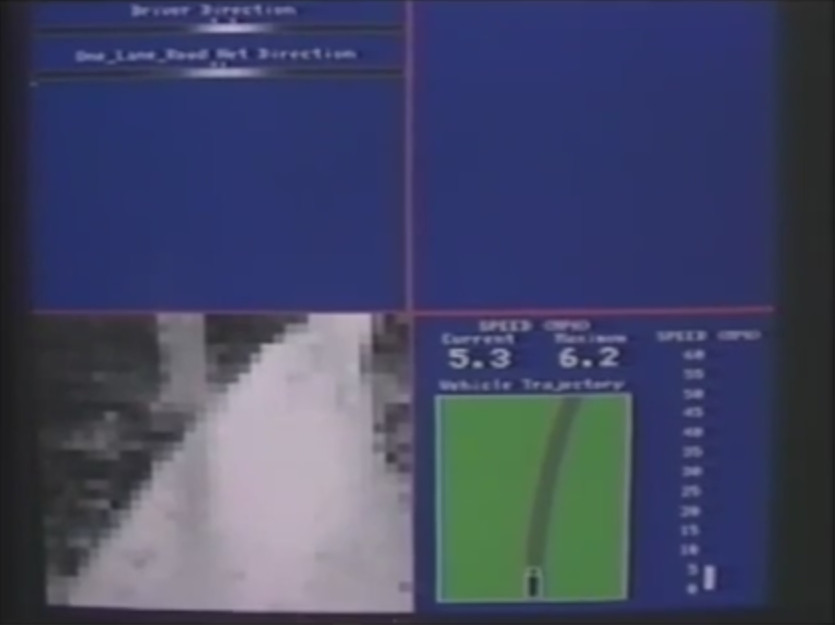
\includegraphics[width=.6\textwidth]{alvinn}
    \caption{Autonomous driving using a neural network\citep{alvinn}\label{fig:alvinn}}
  \end{center}
\end{figure}

\section{Advice for Applying Machine Learning}
When machine learning does not yield good results, it is important to first establish what the problem is before
trying one of the following options
\begin{itemize}
  \item get more training examples
  \item try smaller set of features
  \item try getting additional features
  \item try adding polynomial features
  \item try decreasing $\lambda$
  \item try increasing $\lambda$
\end{itemize}

The data set is separated into a training set (60 \%), cross-validation set (20 \%), and test set (20 \%).
The sum-squared formula (without regularization term) is used to monitor training, to perform cross-validation, and to test the final result:
\begin{itemize}
  \item $J_{train}(\theta)=\frac{1}{2\,m}\,\sumi(h_\theta(\sxi)-\syi)^2$
  \item $J_{cv}(\theta)=\frac{1}{2\,m}\,\sumi(h_\theta(\sxi_{cv})-\syi_{cv})^2$
  \item $J_{test}(\theta)=\frac{1}{2\,m}\,\sumi(h_\theta(\sxi_{test})-\syi_{test})^2$
\end{itemize}
Note that the formulas do not include the regularization term.

Bias (underfit) and high variance (overfit) can be distinguised as follows
\begin{itemize}
  \item \textbf{underfit}: training and validation error both high
  \item \textbf{overfit}: training error low, validation error $>>$ training error
\end{itemize}

The validation data is to select between different models. It can also be used to choose an optimal regularization term. \emph{E.g.} compare $J_{cv}(\theta)$ for $\lambda\in\{0,0.01,0.02,\ldots,10.24\}$.

One can plot the \emph{learning curve} by showing $J_{train}$ and $J_{cv}$ for increasing training set size $m$.
The learning curve allow to detect \emph{bias} and \emph{high variance} more easily
\begin{itemize}
  \item \textbf{high variance}: model not fully converging (curves apart from each other) $\Rightarrow$ get more data or use simpler model
  \item \textbf{bias}: curves quickly converge at a high value and adding more training data does not improve results
\end{itemize}

In summary
\begin{itemize}
  \item get more training examples $\rightarrow$ fixes high variance
  \item try smaller set of features $\rightarrow$ fixes high variance
  \item try getting additional features $\rightarrow$ fixes high bias
  \item try adding polynomial features $\rightarrow$ fixes high bias
  \item try decreasing $\lambda$ $\rightarrow$ fixes high bias
  \item try increasing $\lambda$ $\rightarrow$ fixes high variance
\end{itemize}

When using neural networks, it is generally more effective to use a larger neural network (more hidden units and layers) and address overfitting using regularization (rather than working with a small neural network).
The remaining disadvantage is that larger neural networks are more computationally expensive.

\section{Machine Learning System Design}
\subsection{Prioritizing What to Work On}
Example: Spam email classifier with feature vector ``word $i$ occurs in email or not''.

How to spend your time to make it have low error?
\begin{itemize}
  \item collect lots of data (\emph{e.g.} ``honetpot'' project)
  \item develop sophisticated features based on email routing information (from email header)
  \item develop sophisticated features for message body (\emph{e.g.} should ``discount'' and ``discounts'' be treated as the same word)?
  \item detect deliberate misspellings (\emph{e.g.} m0rtgage, med1cine, w4tches)
\end{itemize}
Instead of randomly fixating on a task, one can use a more systematic way of choosing the next thing to work on.

\subsubsection{Recommended approach}
\begin{itemize}
  \item Start with a simple algorithm that you can implement quickly. Implement it and test it on your cross-validation data.
  \item Plot learning curves to decide if more data, more features, etc. are likely to help.
  \item Error analysis: manually examine the examples (in cross validation set) that your algorithm made errors on.
    See if you spot any systematic trend in what type of examples it is making errors on.
\end{itemize}

It is important to use numerical evaluation, \emph{i.e.} one can quickly evaluate different techniques using the cross validation error. \emph{E.g.} use ``stemming'' or not, distinguish between upper and lower case or not.

In the case of the cancer classification example, only 0.5\% of patients have cancer.
\emph{I.e.} the classification error for the trivial classifier $h(x)=0$ already has 99.5\% accuracy.
In this case the \emph{precision/recall} metric is more appropriate.
\begin{center}
  \begin{tabular}{cc|cc}
    & & \multicolumn{2}{c}{actual class}\\
    &  & 1 & 0\\\hline
    \multirow{2}{*}{predicted class} & 1 & true positive & false positive\\
    & 0 & false negative & true negative\\
  \end{tabular}
\end{center}
Precision and recall are defined as follows:
\begin{itemize}
  \item $precision=\frac{true\ positives}{true\ positives+false\ positives}$ (ratio of true positives and predicted positives)
  \item $recall=\frac{true\ positives}{true\ positives+false\ negatives}$ (ratio of true positives and actual positives)
\end{itemize}

\subsection{Trading of Precision and Recall}
Considering logistic regression $0\le h_\theta(x)\le 1$:
\begin{itemize}
  \item Suppose we want to predict $y=1$ (patient has cancer) only if very confident:
    Predict $1$ if $h_\theta(x)\ge 0.7$ (instead of $0.5$.
    In this case $\Rightarrow$ higher precision, lower recall.
  \item Suppose we want to avoid missing too many cases of cancer (avoid false negatives).
    In this case $\Rightarrow$ higher recall, lower precision.
\end{itemize}
More generally: Predict 1 if $h_\theta(x)\ge threshold$.

To make algorithms comparable, a single number metric, the $F_1$ score is defined:
\begin{equation*}
  F_1\ score=2\frac{P\,R}{P+R}
\end{equation*}

\subsection{Data For Machine Learning}
\citep{banko2001scaling} shows that data trumps algorithms:
``It’s not who has the best algorithms who wins, it’s who has the most data.''

Sometimes more features are required rather than more samples.

A useful test is: ``Given the input $x$, can a human expert confidently predict $y$?''

Using a large training set ensures low variance. \emph{I.e.} $J_{train}(\theta)\approx J_{test}(\theta)$.
This allows using a learning algorithm with many parameters so that $J_{test}(\theta)$ will be small.

\section{Support Vector Machines}
\subsection{Optimization Objective}
\acp{SVM} can be a powerful method for solving supervised learning problems.
Logistic regression uses
\begin{equation*}
  h_\theta(x)=\frac{1}{1+\operatorname{e}^{-\theta^\top x}}
\end{equation*}
\begin{itemize}
  \item if $y=1$, we want $h_\theta(x)\approx 1$, $\theta^\top x\gg0$
  \item if $y=0$, we want $h_\theta(x)\approx 0$, $\theta^\top x\ll0$
\end{itemize}
For $y=1$ the cost term is (also see Figure \ref{fig:logcost})
\begin{equation*}
  -\operatorname{log}\frac{1}{1+\operatorname{e}^{-\theta^\top x}}
\end{equation*}
\begin{figure}[htbp]
  \begin{center}
    \includegraphics[width=.4\textwidth]{logcost}
    \caption{Cost terms for $y=1$ and $y=1$ with $\theta=1$\label{fig:logcost}}
  \end{center}
\end{figure}

The cost function of logistic regression is
\begin{equation*}
  \mathop{\operatorname{min}}_\theta\frac{1}{m}\bigg[\sumi\syi\big(-\operatorname{log}h_\theta(\sxi)\big)+(1-\syi)\big(-\operatorname{log}(1-h_\theta(\sxi)\big)\bigg]+\frac{\lambda}{2\,m}\sum_{j=1}^n\theta_j^2
\end{equation*}
The \ac{SVM} uses a modified cost function
\begin{equation*}
  \mathop{\operatorname{min}}_\theta C\bigg[\sumi\syi cost_1(\theta^T\sxi)+(1-\syi)cost_0(\theta^\top\sxi)\bigg]+\frac{1}{2}\sum_{j=1}^n\theta_j^2
\end{equation*}
The parameter $C$ is used instead of $\frac{1}{\lambda}$ to control the regularization trade-off.

A \ac{SVM} does not output a probability. Instead it just makes a prediction:
\begin{equation*}
  h_\theta(x)=\left\{\begin{array}{rl}1&\mathrm{if }\theta^\top x\ge 0\\0&\mathrm{otherwise}\end{array}\right.
\end{equation*}
The constant offset $\theta_0$ is realised using $x_0=1$.

\subsection{Large Margin Intuition}
\acp{SVM} use the following non-differentiable terms for defining the cost function:
\begin{align*}
  \begin{split}
    cost_1(z)&=\operatorname{max}(1-z,0)\\
    cost_0(z)&=\operatorname{max}(z+1,0)
  \end{split}
\end{align*}
\begin{itemize}
  \item if $y=1$, we want $h_\theta(x)=1$, $\theta^\top x\ge 1$
  \item if $y=0$, we want $h_\theta(x)=0$, $\theta^\top x\le -1$
\end{itemize}
The \ac{SVM} will try to find a decision boundary which has a distance from the labelled data.
\ac{SVM} can give you a \emph{large margin classifier} which is more robust.

\subsection{Mathematics behind Large Margin Classification}
The regularization objective is to minimize
\begin{equation*}
  \frac{1}{2}\sum_j^n\theta_j^2
\end{equation*}
\emph{i.e.} to keep the norm of the parameter vector $||\theta||$ small.
Assuming the simplified case $\theta_0=0$, the objective of the cost function is to keep
\begin{align*}
  \begin{split}
    p^{(i)}\cdot||\theta||\ge 1&\mathrm{\ if\ }y^{(i)}=1\\
    p^{(i)}\cdot||\theta||\le -1&\mathrm{\ if\ }y^{(i)}=0
  \end{split}
\end{align*}
small, where $p^{(i)}$ is the projection of $\sxi$ onto the vector $\theta$.
\emph{I.e.} if the achievable margin is small, $||\theta||$ must be large.
If the margin is large, $||\theta||$ can be smaller.

When $\theta_0\ne 0$, there is a generalisation of this argument that shows, that the same holds for decision boundaries not passing through the origin.

\clearpage

\appendix
\section{Appendix}
\subsection{Least Squares Estimator}\label{app:lse}
\inputminted[frame=lines,linenos,fontsize=\small]{python}{least_squares.py}

\subsection{Linear Regression}\label{app:gradientdescent}
\inputminted[frame=lines,linenos,fontsize=\small]{python}{gradient_descent.py}

\subsection{Learning Rate}\label{app:alphas}
\inputminted[frame=lines,linenos,fontsize=\small]{python}{learning_rate.py}

\subsection{Logistic Regression}\label{app:classifier}
\inputminted[frame=lines,linenos,fontsize=\small]{python}{classifier.py}

\subsection{Polynomial Features}\label{app:polynomial}
\inputminted[frame=lines,linenos,fontsize=\small]{python}{polynomial.py}

\subsection{Overfitting Example}\label{app:overfitting}
\inputminted[frame=lines,linenos,fontsize=\small]{python}{overfitting.py}

\subsection{Backpropagation using Theano}\label{app:backprop}
Backpropagation example from \url{https://stackoverflow.com/questions/44210561/how-do-backpropagation-works-in-tensorflow}
\inputminted[frame=lines,linenos,fontsize=\small]{python}{backprop.py}

\subsection{Backpropagation applied to the MNIST Dataset}\label{app:mnistbackprop}
\inputminted[frame=lines,linenos,fontsize=\small]{python}{mnist-backprop.py}

\subsection{Convolution using Theano}
\inputminted[frame=lines,linenos,fontsize=\small]{python}{convolution.py}

\section{References and Glossary}
\subsection{References}
\printbibliography[heading=none]

\subsection{Glossary}
\begin{acronym}[L-BFGS]
  \acro{BFGS}{Broyden-Fletcher-Goldfarb-Shanno algorithm}
  \acro{L-BFGS}{Limited-memory BFGS}
  \acro{SVM}{Support Vector Machine}
\end{acronym}

\end{document}
